\documentclass[journal,12pt,twocolumn]{IEEEtran}

\usepackage{setspace}
\usepackage{gensymb}
\singlespacing
\usepackage{amsmath}
\usepackage{amsthm}
\usepackage{comment}
\usepackage{mathrsfs}
\usepackage{txfonts}
\usepackage{stfloats}
\usepackage{bm}
\usepackage{cite}
\usepackage{cases}
\usepackage{subfig}

\usepackage{longtable}
\usepackage{multirow}

\usepackage{enumitem}
\usepackage{mathtools}
\usepackage{steinmetz}
\usepackage{tikz}
\usepackage{circuitikz}
\usepackage{verbatim}
\usepackage{tfrupee}
\usepackage[breaklinks=true]{hyperref}
\usepackage{graphicx}
\usepackage{tkz-euclide}

\usetikzlibrary{calc,math}
\usetikzlibrary{automata, positioning}
\usepackage{listings}
    \usepackage{color}                                            %%
    \usepackage{array}                                            %%
    \usepackage{longtable}                                        %%
    \usepackage{calc}                                             %%
    \usepackage{multirow}                                         %%
    \usepackage{hhline}                                           %%
    \usepackage{ifthen}                                           %%
    \usepackage{lscape}     
\usepackage{multicol}
\usepackage{chngcntr}

\DeclareMathOperator*{\Res}{Res}

\renewcommand\thesection{\arabic{section}}
\renewcommand\thesubsection{\thesection.\arabic{subsection}}
\renewcommand\thesubsubsection{\thesubsection.\arabic{subsubsection}}

\renewcommand\thesectiondis{\arabic{section}}
\renewcommand\thesubsectiondis{\thesectiondis.\arabic{subsection}}
\renewcommand\thesubsubsectiondis{\thesubsectiondis.\arabic{subsubsection}}


\hyphenation{op-tical net-works semi-conduc-tor}
\def\inputGnumericTable{}                                 %%

\lstset{
%language=C,
frame=single, 
breaklines=true,
columns=fullflexible
}

\begin{document}

\newcommand{\BEQA}{\begin{eqnarray}}
\newcommand{\EEQA}{\end{eqnarray}}
\newcommand{\define}{\stackrel{\triangle}{=}}
\bibliographystyle{IEEEtran}
\raggedbottom
\setlength{\parindent}{0pt}
\providecommand{\mbf}{\mathbf}
\providecommand{\pr}[1]{\ensuremath{\Pr\left(#1\right)}}
\providecommand{\qfunc}[1]{\ensuremath{Q\left(#1\right)}}
\providecommand{\sbrak}[1]{\ensuremath{{}\left[#1\right]}}
\providecommand{\lsbrak}[1]{\ensuremath{{}\left[#1\right.}}
\providecommand{\rsbrak}[1]{\ensuremath{{}\left.#1\right]}}
\providecommand{\brak}[1]{\ensuremath{\left(#1\right)}}
\providecommand{\lbrak}[1]{\ensuremath{\left(#1\right.}}
\providecommand{\rbrak}[1]{\ensuremath{\left.#1\right)}}
\providecommand{\cbrak}[1]{\ensuremath{\left\{#1\right\}}}
\providecommand{\lcbrak}[1]{\ensuremath{\left\{#1\right.}}
\providecommand{\rcbrak}[1]{\ensuremath{\left.#1\right\}}}
\theoremstyle{remark}
\newtheorem{rem}{Remark}
\newcommand{\sgn}{\mathop{\mathrm{sgn}}}
\providecommand{\abs}[1]{\vert#1\vert}
\providecommand{\res}[1]{\Res\displaylimits_{#1}} 
\providecommand{\norm}[1]{\lVert#1\rVert}
%\providecommand{\norm}[1]{\lVert#1\rVert}
\providecommand{\mtx}[1]{\mathbf{#1}}
\providecommand{\mean}[1]{E[ #1 ]}
\providecommand{\fourier}{\overset{\mathcal{F}}{ \rightleftharpoons}}
%\providecommand{\hilbert}{\overset{\mathcal{H}}{ \rightleftharpoons}}
\providecommand{\system}{\overset{\mathcal{H}}{ \longleftrightarrow}}
	%\newcommand{\solution}[2]{\textbf{Solution:}{#1}}
\newcommand{\solution}{\noindent \textbf{Solution: }}
\newcommand{\cosec}{\,\text{cosec}\,}
\providecommand{\dec}[2]{\ensuremath{\overset{#1}{\underset{#2}{\gtrless}}}}
\newcommand{\myvec}[1]{\ensuremath{\begin{pmatrix}#1\end{pmatrix}}}
\newcommand{\mydet}[1]{\ensuremath{\begin{vmatrix}#1\end{vmatrix}}}
\numberwithin{equation}{subsection}
\makeatletter
\@addtoreset{figure}{problem}
\makeatother
\let\StandardTheFigure\thefigure
\let\vec\mathbf
\renewcommand{\thefigure}{\theproblem}
\def\putbox#1#2#3{\makebox[0in][l]{\makebox[#1][l]{}\raisebox{\baselineskip}[0in][0in]{\raisebox{#2}[0in][0in]{#3}}}}
     \def\rightbox#1{\makebox[0in][r]{#1}}
     \def\centbox#1{\makebox[0in]{#1}}
     \def\topbox#1{\raisebox{-\baselineskip}[0in][0in]{#1}}
     \def\midbox#1{\raisebox{-0.5\baselineskip}[0in][0in]{#1}}
\vspace{3cm}
\title{Assignment 4- Probability and Random Variables}
\author{Songa Kotesh Satvik}
\maketitle
\newpage
\bigskip
\renewcommand{\thefigure}{\theenumi}
\renewcommand{\thetable}{\theenumi}
Download all python codes from 
\begin{lstlisting}
https://github.com/KoteshSatvik/AI1103-Probability_and_Random_Variables/tree/main/Assignment-4/codes
\end{lstlisting}
%
and latex-tikz codes from 
%
\begin{lstlisting}
https://github.com/KoteshSatvik/AI1103-Probability_and_Random_Variables/blob/main/Assignment-4/Assignment4.tex
\end{lstlisting}
\section{\textbf{Gate 2016 (cs-set 1) Q:}29}
Consider the following experiment.\\
\textbf{Step 1.} Flip a fair coin twice.\\
\textbf{Step 2.} If the outcomes are (TAILS, HEADS) then output Y and stop.\\
\textbf{Step 3.} If the outcomes are either (HEADS, HEADS) or (HEADS, TAILS), then output N and stop.\\
\textbf{Step 4.} If the outcomes are (TAILS, TAILS), then go to Step 1.\\
The probability that the output of the experiment is Y is (upto two decimal places)
\section{\textbf{Solution}}
Given a fair coin is flipped twice. Let us represent the outcome as (x,y) where x represents the outcome in first throw and y represents the outcome in the second throw.\\
\begin{table}[hbt!]
\resizebox{\columnwidth}{!}{
\begin{tabular}{|c|l|}
\hline
\textbf{Variable} & \multicolumn{1}{c|}{\textbf{Event}}          \\ \hline
S                 & Event of tossing a fair coin twice           \\ \hline
N                 & Event of obtaining 'N' as the output         \\ \hline
Y                 & Event of obtaining 'Y' as the output         \\ \hline
T                 & Event of obtaining (TAIL,TAIL) as the output \\ \hline
\end{tabular}
}
\caption{Variables representing different events}
\label{table:1}
\end{table}

When a fair coin is tossed twice the output is, \\
'N' when the outcomes are (H,H), (H,T) and\\
'Y' when the outcome is (T,H).\\
Then, \\
\textbf{Markov chain diagram :}\\
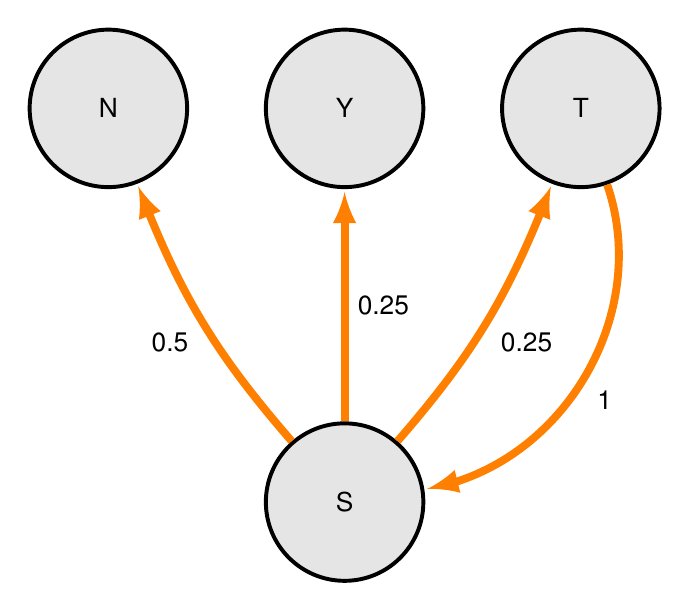
\begin{tikzpicture}[font=\sffamily]

        % Setup the style for the states
        \tikzset{node style/.style={state, 
                                    minimum width=2cm,
                                    line width=0.5mm,
                                    fill=gray!20!white}}

        % Draw the states
        \node[node style] at (1, 0)     (N)     {N};
        \node[node style] at (4, 0)     (Y)     {Y};
        \node[node style] at (7, 0)     (T)     {T};
        \node[node style] at (4, -5)    (S)     {S};
        
        % Connect the states with arrows
        \draw[every loop,
              auto=right,
              line width=1mm,
              >=latex,
              draw=orange,
              fill=orange]
            (S)     edge[bend left=10, auto=left]  node {0.5} (N)
            (S)     edge                node {0.25} (Y)
            (S)     edge[bend right=10, auto=right] node {0.25} (T)
            (T)     edge[bend left=50, auto=left]            node {1} (S)
            ;
\end{tikzpicture}

\textbf{Let :} $X_0$ be defined as the initial state (at time 0). \\
\textbf{Given :} Initial state is 'S'($X_0$)\\
\textbf{To find :} Probability of outcome being Y.\\
Therefore we have to find the probability of absorption in state Y.\\
Let us define,
\begin{align}
    a_i &= \pr{\text{final state is Y$|X_0$ = i}}\\
\shortintertext{Therefore by definition,}
    a_Y &= 1\\
    a_N &= 0\\
    a_T &= a_S\\
    a_S &=  \frac{1}{4}[a_Y + a_T] + \frac{1}{2}(a_N)\\
    \implies a_S &= \frac{1}{4}a_Y + \frac{1}{4}a_T\\
    \implies a_S &= \frac{1}{4}a_Y + \frac{1}{4}a_S\\
    \implies \frac{3}{4}a_S &= \frac{1}{4}a_Y\\
    \therefore a_S &= \frac{1}{3}    
\end{align}
Therefore the probability of outcome being Y is 0.33 (rounded to two decimal places).
\end{document}